\chapter{Experiments and Results}
\label{AER}

\section{Graph Behavior}
\Cref{tab:results:graph_behavior} elaborates how a change in parameter value changes the shape and population level of the agents. 
"\nameref{sec:results:a_good_curve}", whose agent and parameter default values can be found in the first column of \Cref{tab:results:graph_behavior} and in \Cref{tab:appendixE:a_good_curve} are used as a reference. 
Each parameter was individually changed to a higher and lower value from the reference value, and the changes were noted in \Cref{tab:results:graph_behavior}. 
It should be noted that \Cref{tab:results:graph_behavior} provides illustrative examples rather than an exhaustive analysis. The observed behaviors reflect typical trends when varying each parameter in the indicated direction, but may not generalize to all possible values and cases, or the magnitude of the change. 
The results can also not be generalized to cases where two parameters values are changed at a time. 
\Cref{tab:results:graph_behavior} can be used in conjunction with \nameref{sec:SOBOL_sensitivity_analysis_results} to gain a better idea of how sensitive the output is to that specific parameter. 

\begin{table}
    \small % or \footnotesize to make it more compact
    \centering
    \begin{tabularx}{\textwidth}{l l X}
        \toprule
        \textbf{Parameter} & \textbf{Tested Value} & \textbf{Description of Behavior} \\
        \midrule
        $R$ (400) & 500 & More uninfected and infected, slightly more phages\\
         & 300 & Slightly less uninfected and infected, earlier resource depletion\\

        \midrule
        $U$ (50) & 70 & Slightly more phages and uninfected and infected bacteria\\
         & 30 & Less uninfected and infected bacteria, slower resource depletion, not all resources used, slightly less phages \\

        \midrule
        $P$ (10) & 20 & Less resources consumed, less uninfected, bacteria peaks earlier, slightly less phages\\
         & 5 & Resources consumed faster, more uninfected, infected, and phages\\

        \midrule
        $\tau$ (2.14) & 10 & Faster resource depletion, faster bacteria peak, plateau, then fall in population. more uninfected and infected, less phages\\
         & 0.5& Barely any resource consumption, little bacteria growth and uninfected, more phages\\

        \midrule
        $\omega^i$ (0) & 15 & Slightly more bacteria, resource replenish after bacteria die out\\

        \midrule
        $e$ (0.03) & 0.1 & Faster resource depletion, sharper decline in uninfected, less infected and phages \\
         & 0.01 & Less resource consumption, slightly more bacteria\\

        \midrule
        $v$ (1.2) & 1.8 & More phages, significantly more bacteria, earlier and sharp peak in uninfected, , \\
         & 1 & Less phages and bacteria, less resource consumption, earlier bacteria peak\\

        \midrule
        $K$ (10) & 100 & Less resource consumption, less bacteria and phages, earlier bacteria peak\\
         & 1 & Faster resource depletion and sudden stop instead of gradual slowdown, earlier bacteria peak\\

        \midrule
        $r$ (0.01) & 0.1 & Less consumption, less infected and phages, earlier peak in bacteria\\
         & 0.001 & Faster resource consumption rate, more infected and phages, delay in bacteria peak, sharp bacteria peak, small plateau in bacteria count before drop\\

        \midrule
        $\beta$ (20) & 50 & More phages, earlier bacteria peak, less resources consumed, less bacteria\\
         & 10 & Faster resource consumption, more uninfected, less phages, sharper bacteria peak\\

        \midrule
        $\omega^o$ (0) & 0.02 & Faster resource depletion, more bacteria and sharper peak, later peak, and less phages. \\

        \bottomrule
    \end{tabularx}
    \caption{
        A table that compares how moving one individual parameter value up or down relative to the "\nameref{sec:results:a_good_curve}" changes the general shape of the curve. 
        This table is not meant to be exhaustive, cover edge cases, or extreme cases, or cover every exact detail and change in the population graph, but just to give an idea of how a change in parameter influences the graph shape, such as the rate of resource depletion, maximum number of bacteria and phages, and change in peak time. 
        Reference parameter values are provided in the parentheses, from \Cref{tab:appendixE:a_good_curve}. 
    }
    \label{tab:results:graph_behavior}
\end{table}


\section{A Good Curve}
\label{sec:results:a_good_curve}
Assuming a very simple model, with no washin or washout rate, a good bacteria growth curve looks like a mountain, with a clear rise, peak, and fall in population levels. 
For a given IC, the bacteria start to consume resources and replicate leading to exponential growth. 
The phages start to infect the bacteria and eventually the bacteria start to die, releasing new phages. 
The new phages infect more bacteria, putting pressure on the bacteria growth. 
Eventually, more bacteria are being infected than being created, causing the decline in bacteria population. 
\Cref{fig:created:a_good_curve_linear} shows an example of a good curve. 
\Cref{fig:created:a_good_curve_logarithmic} is the same plot but with a logarithmic y-axis. 

As the bacteria population grow, the resource consumption speeds up until there are trace amount of resources left at $t=8$. 
The uninfected and infected bacteria exhibit exponential growth, peaking at 1617 at $t=3.99$ and 3463 at $t=5.27$ respectively. 
The delay in the uninfected to infected bacteria's peak is due to the infection stages and latent period of the phage infection. 
The bacteria sum do not have as stark of a peak in comparison to the uninfected and infected bacteria, due to the graph measuring all bacteria populations, but the peak of 3805 at $t=4.89$ is still clear. 
The phages saw a significant increase in population count at around $t=4$, coinciding with the peak in uninfected bacteria. 
At this point in time, the infection rate is larger than the bacteria replication rate, so the bacteria are starting to die out even though there are still sufficient resources remaining. 
At around $t=4$ is when the the resource consumption rate inflects. 
The rate at which the resources are being consumed starts to slow down, showing a decreasing sigmoid shape. 
The total bacteria population reached a peak of 3805 at $t=4.89$, a 76.1x increase in population count from the initial 50 starting uninfected bacteria. 
The phage population reached a peak of 2584 phages at $t=15$, a 258.4x increase in population count. 

\begin{figure}[h!]
    \centering
    \begin{subfigure}{1\linewidth}
        \centering
        \captionsetup{width=1\linewidth}
        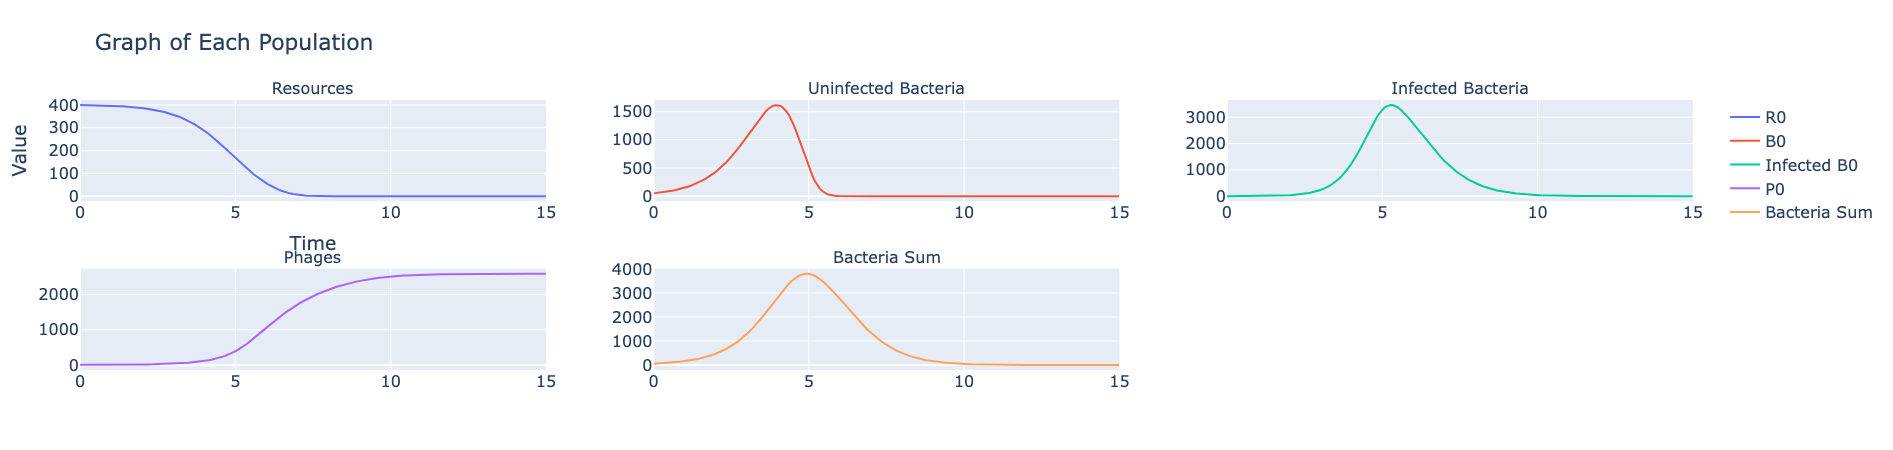
\includegraphics[width=\linewidth]{Plots/Created/a_good_curve_linear.png}
        \caption{
            Linear y-axis for a "good" plot. 
        }
        \label{fig:created:a_good_curve_linear}
    \end{subfigure}
    \hfill
    \begin{subfigure}{1\linewidth}
        \centering
        \captionsetup{width=1\linewidth}
        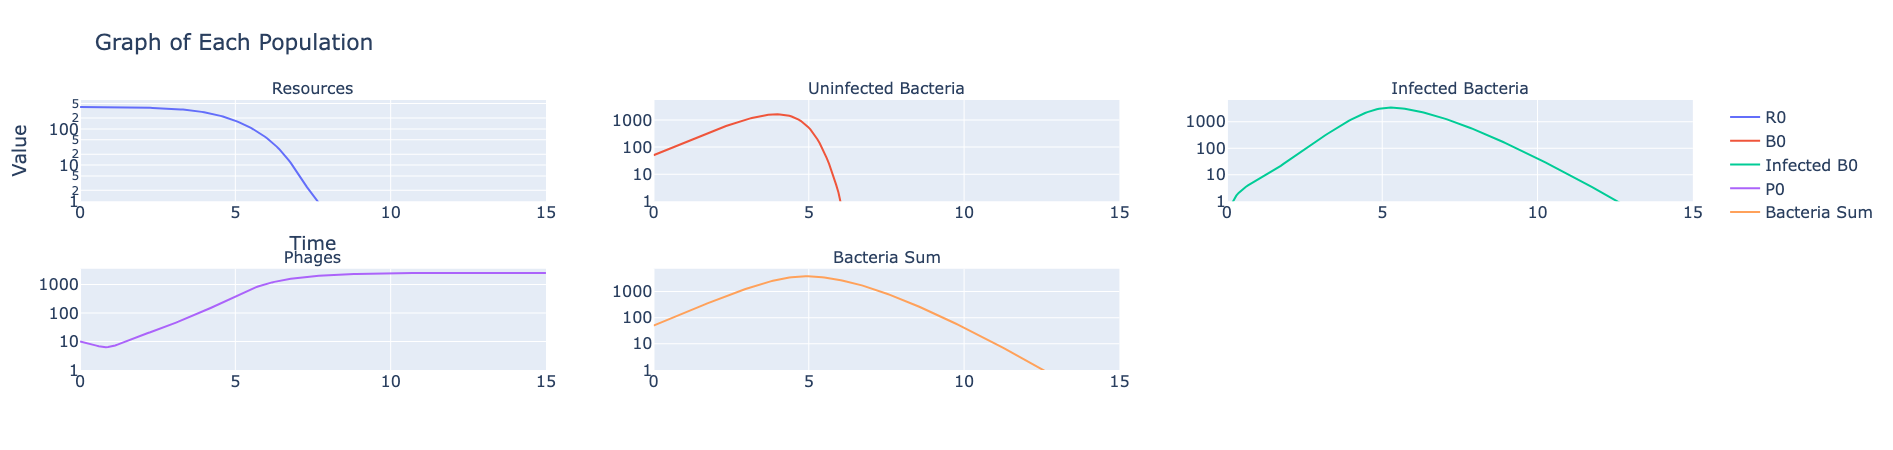
\includegraphics[width=\linewidth]{Plots/Created/a_good_curve_logarithmic.png}
        \caption{
            Logarithmic y-axis for a "good" plot. 
        }
        \label{fig:created:a_good_curve_logarithmic}
    \end{subfigure}
    \caption{
        The log plot allows to see behavior happening at values near 0 and to plot data on a logarithmic scale. 
        The parameters used for this plot can be found in \Cref{tab:appendixE:a_good_curve}. 
    }
    \label{fig:created:a_good_curve}
\end{figure}

\section{SOBOL Sensitivity Analysis Results}
\label{sec:SOBOL_sensitivity_analysis_results}
It is important to understand how a change in parameter value affects the change in output of a model. 
Models will have parameters that are more important and have a larger effect on the model output than other parameters. 

\Cref{fig:created:SOBOL_final} shows the impact that the parameter had on the final value of the population at $t=15$. 
THe average value and variance of population value were intentionally left out of the analysis, despite being a part of the dashboard because the SOBOL sensitivity values are almost identical to the final sensitivity values. 
There were some very minor differences from bar to bar across plots, but the difference was imperceptible. 
Since the plots all look similar, only an analysis on the final value, \Cref{fig:created:SOBOL_final} will be done. 

The parameters that were tested include all the parameters listed in the extended golden model, except for Uninfected Bacteria and $M$. 
Uninfected Bacteria was left out as it doesn't make sense to already add infected bacteria to the system
$M$, the number of stages that the infection goes through, can not be tested as $M$ hardcodes the number of infection stages that the bacteria has to go through. 
The hardcoding is done before the simulation framework starts. 
As such, it is not possible to change $M$. 

\subsection{Final Value Analysis}
\subsubsection{Resources}
The $\omega^i$/washin rate had the largest influence on the final, average and variance value. 
Without a washin rate, the resources will most likely have been consumed by the time the simulation ended at $t=15$. 
The final values for Resources, Uninfected, Infected, and Phages would often be something similar to (0, 0, 0, 10000) at $t=15$, where all the resources were consumed and the bacteria died out due to the phages, leaving only the phages remaining. 
The final value of the resources would often be 0, no matter what parameter values were used, with $\omega^i, \omega^o = 0$. 
With the addition of the washin, new resources were constantly being re-added. 
Once the bacteria died out, the resources could accumulate, with the accumulation dependent on the rate of the washin rate, hence why the washin rate has such a large impact on the final, average, and variance of population value for the resources. 
The final value would be dependent on when the bacteria died out, in turn allowing the resources to accumulate at a rate proportional to $\omega^i - \omega^0\cdot R$. 
Resources were less dependent on higher order interactions, unlike the uninfected, infected, phages, and total bacteria sum. 

\subsubsection{Uninfected}
The uninfected bacteria population sensitivities depend on many higher order interactions between the parameters as $ST_i >> S1_i$. 
The uninfected are highly dependent on $\beta$/B\_matrix and initial phage population, as the initial phage population will determine how many bacteria become infected, and how quickly the phages can proliferate through the bacteria population. 
Surprisingly, $r$/r\_matrix did not have as big of an influence on the uninfected as $\beta$ did, even though the infection rate is dependent on $r$. 
The larger or smaller $r$ is, the faster or slower the infection rate is. If $r$ is really small, the infection rate would take forever, potentially allowing the bacteria to keep a stable population. 
$r$ is equally as important at explaining the final value as $\tau$/tau\_vector, washin, $e$/e\_matrix, and washout of sensitivity around 0.25. 

\subsubsection{Infected}
Since $ST_i >> S1_i$ for the infected bacteria, where $S1_i \approx 0$ for nearly all of the parameters, the infected bacteria heavily depend on many interactions happening at the same time. 
This makes intuitive sense after looking at \nameref{sec:golden_model}. 
The infected (and uninfected) bacteria directly interact with $R$, $U$, $P$, $v$, $K$, $r$, $\tau$, and $\omega^o$ ($M$ is not included as it was left out of the analysis). 
So due to the high coupling of parameters, the infected (and also the uninfected) have large global sensitivities compared to the local sensitivity. 

However SOBOL had some difficulties assigning a good sensitivity score to each parameter for the $ST$ and $S1$ tests as noticed by the slightly larger error bars in the infected than the uninfected or resources. 
This is most likely due to the infected bacteria going through multiple stages of infection, causing a delay and uncertain behavior in the final value, despite the ODE model being deterministic. 

\subsubsection{Phages}
The most important factor for the final phage value is $r$, followed by $\beta$, $\omega^o$ and $P$. 
The $r$ value allows the phages to infect the uninfected. 
When $r$ is decreased, the final phage population is counterintuitively higher than when $r$ is larger. 
The behavior is counterintuitive because one would expect that a higher infection rate would lead to more infections and thus more phages. 
With a higher $r$ value, more phages are being removed from the phage population and infecting the bacteria. 
It can be seen as a way of "more phages are needed to infect a bacterium", therefore getting less phages out as a result as more phages are needed to infect a single bacteria. 

Washout has a noticeable influence on the phage population, as not the phage population is being reduced at a rate proportional to the washout rate. 
The larger the washout rate, the larger the drawdown of phages. 
When the infected all die out, the phage population wont grow anymore. 
Given the phage population at that point in time, the phage removal rate is proportional to the washout rate. 

\subsubsection{Total Bacteria}
Total bacteria is the sum of both uninfected and infected bacteria, so it makes sense for total bacteria to have similar values to uninfected and infected bacteria. 
Apparently the uninfected bacteria have a stronger influence on the output variance than the infected bacteria. 
The total bacteria sensitivities resemble the sensitivities of the uninfected bacteria more than the infected bacteria. 
It would have been expected for the total bacteria to resemble more of an average between the uninfected and infected. 

\begin{figure}[h!]
    \centering
    \begin{subfigure}{0.32\linewidth}
        \centering
        \captionsetup{width=1\linewidth}
        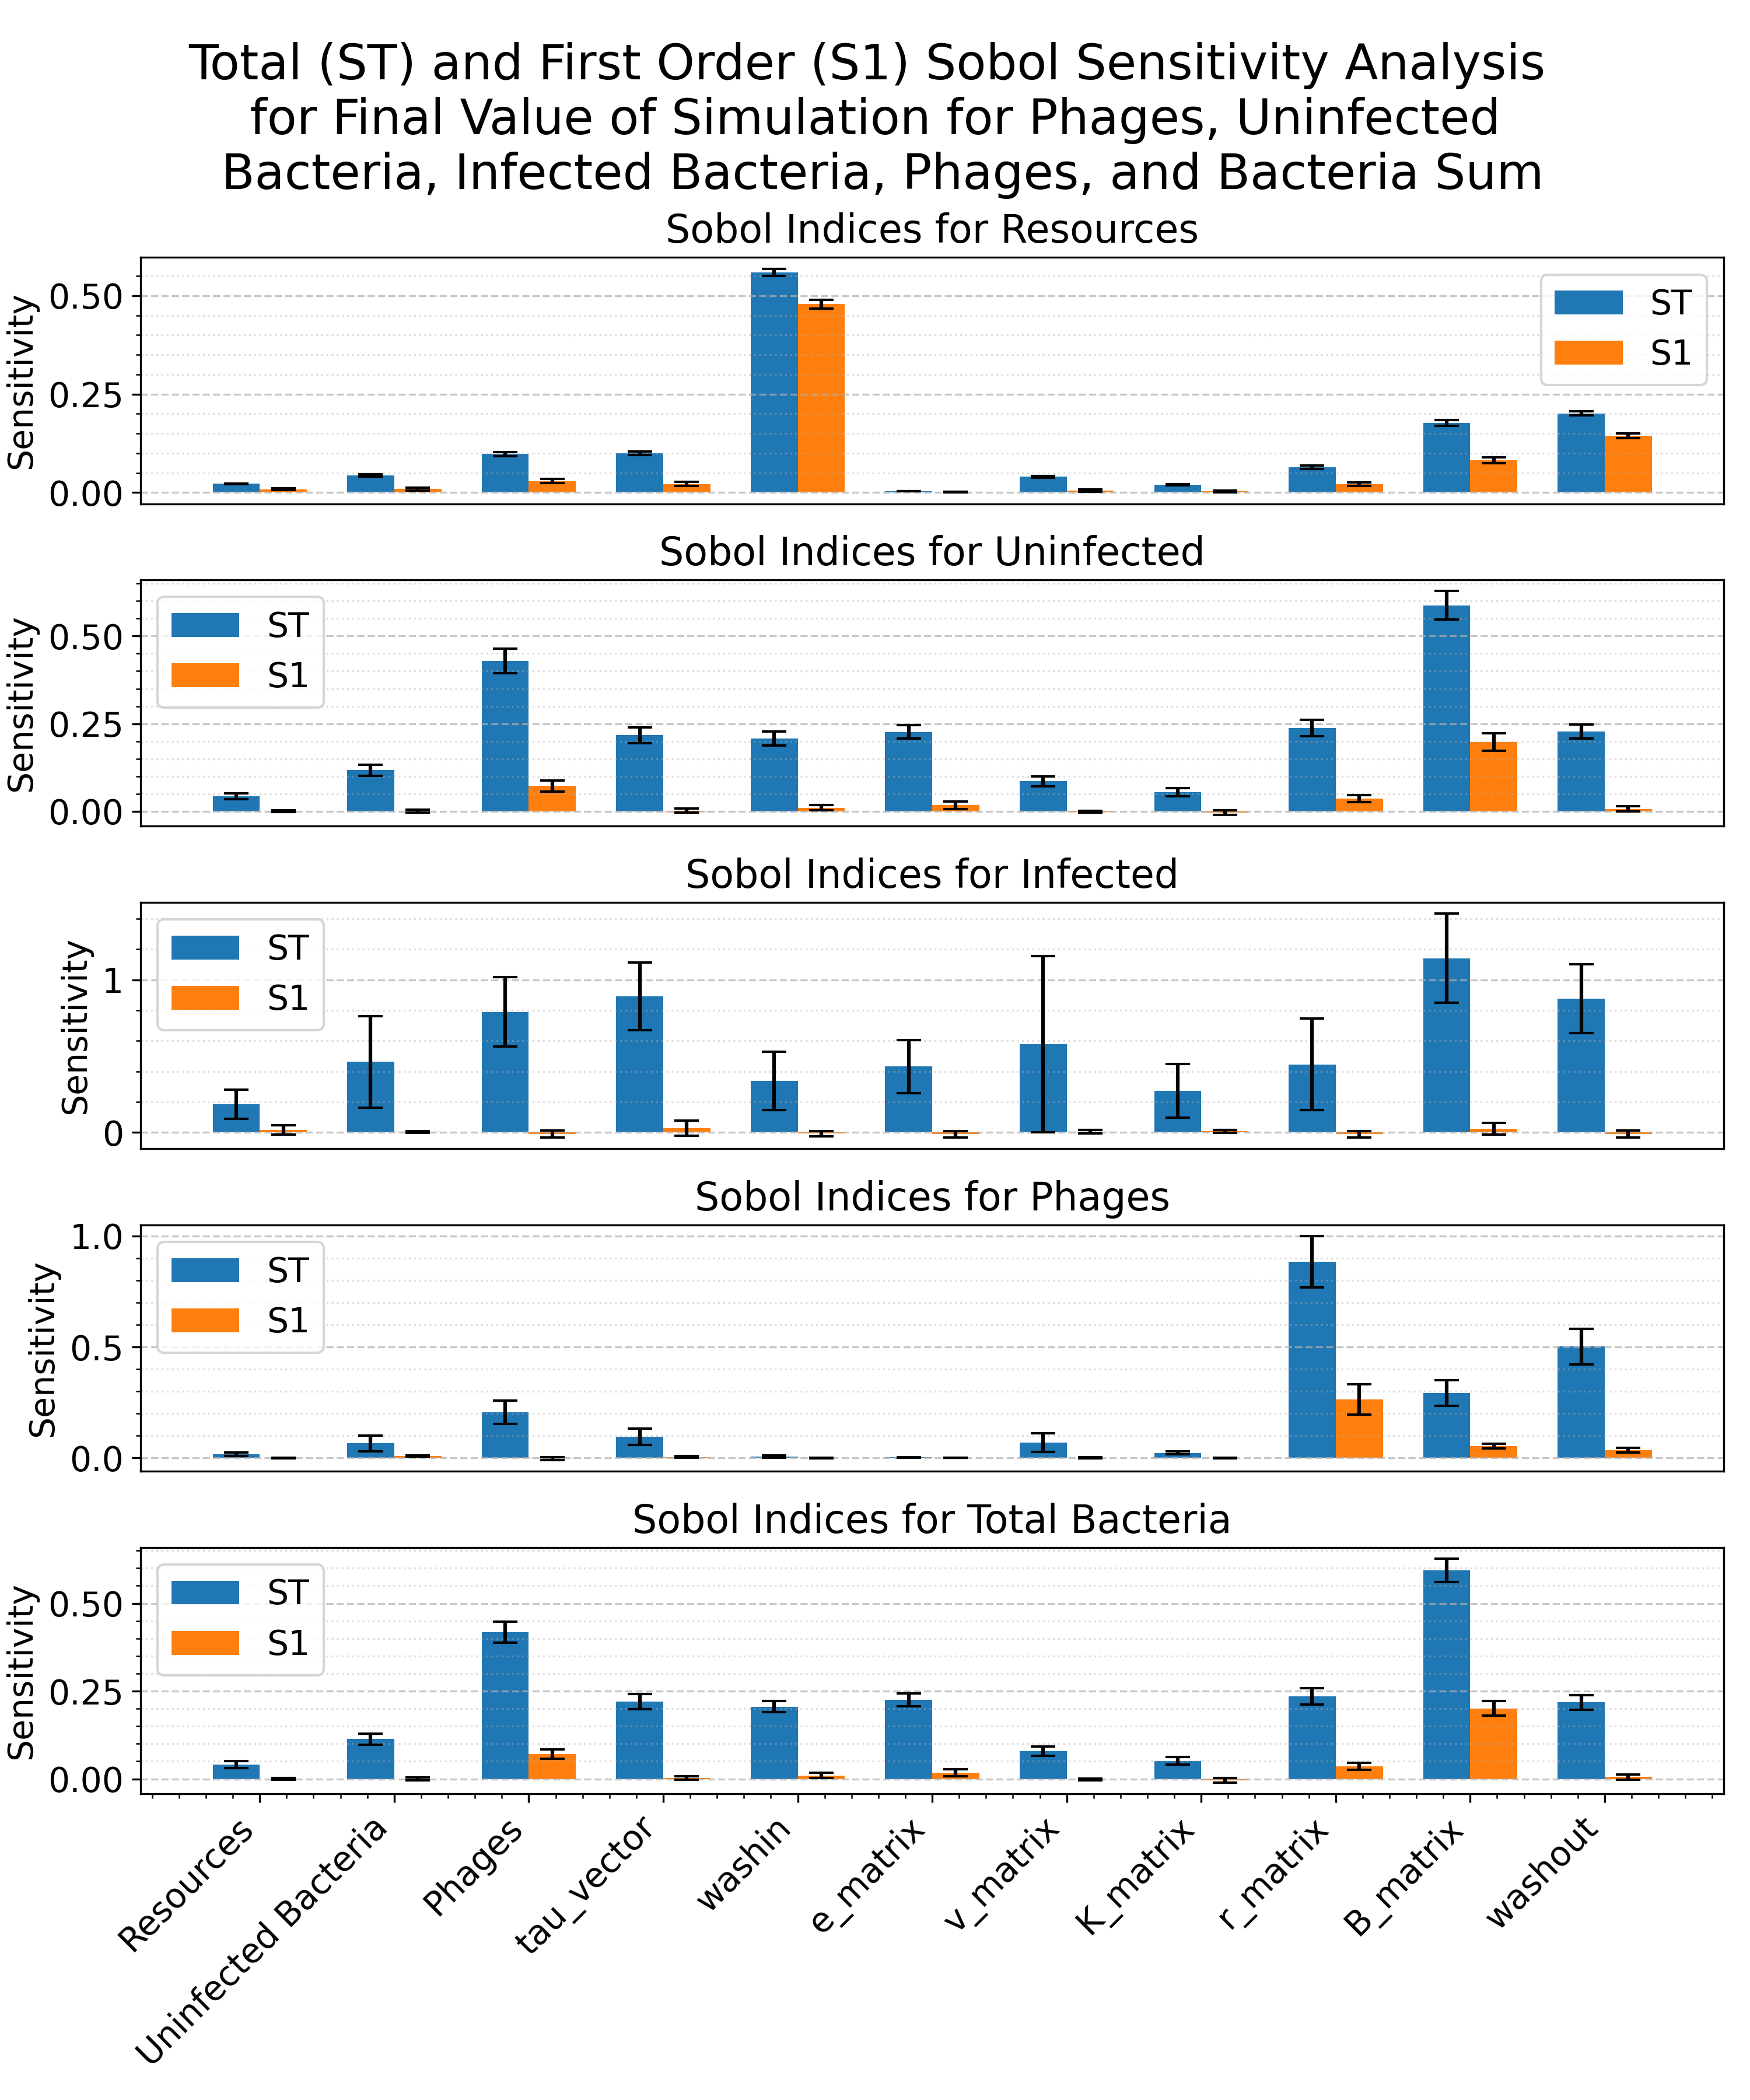
\includegraphics[width=\linewidth]{Plots/Created/SOBOL/SOBOL_analysis_1748084143_Final.png}
        \caption{
            Final population value. 
        }
        \label{fig:created:SOBOL_final}
    \end{subfigure}
    \hfill
    \begin{subfigure}{0.32\linewidth}
        \centering
        \captionsetup{width=1\linewidth}
        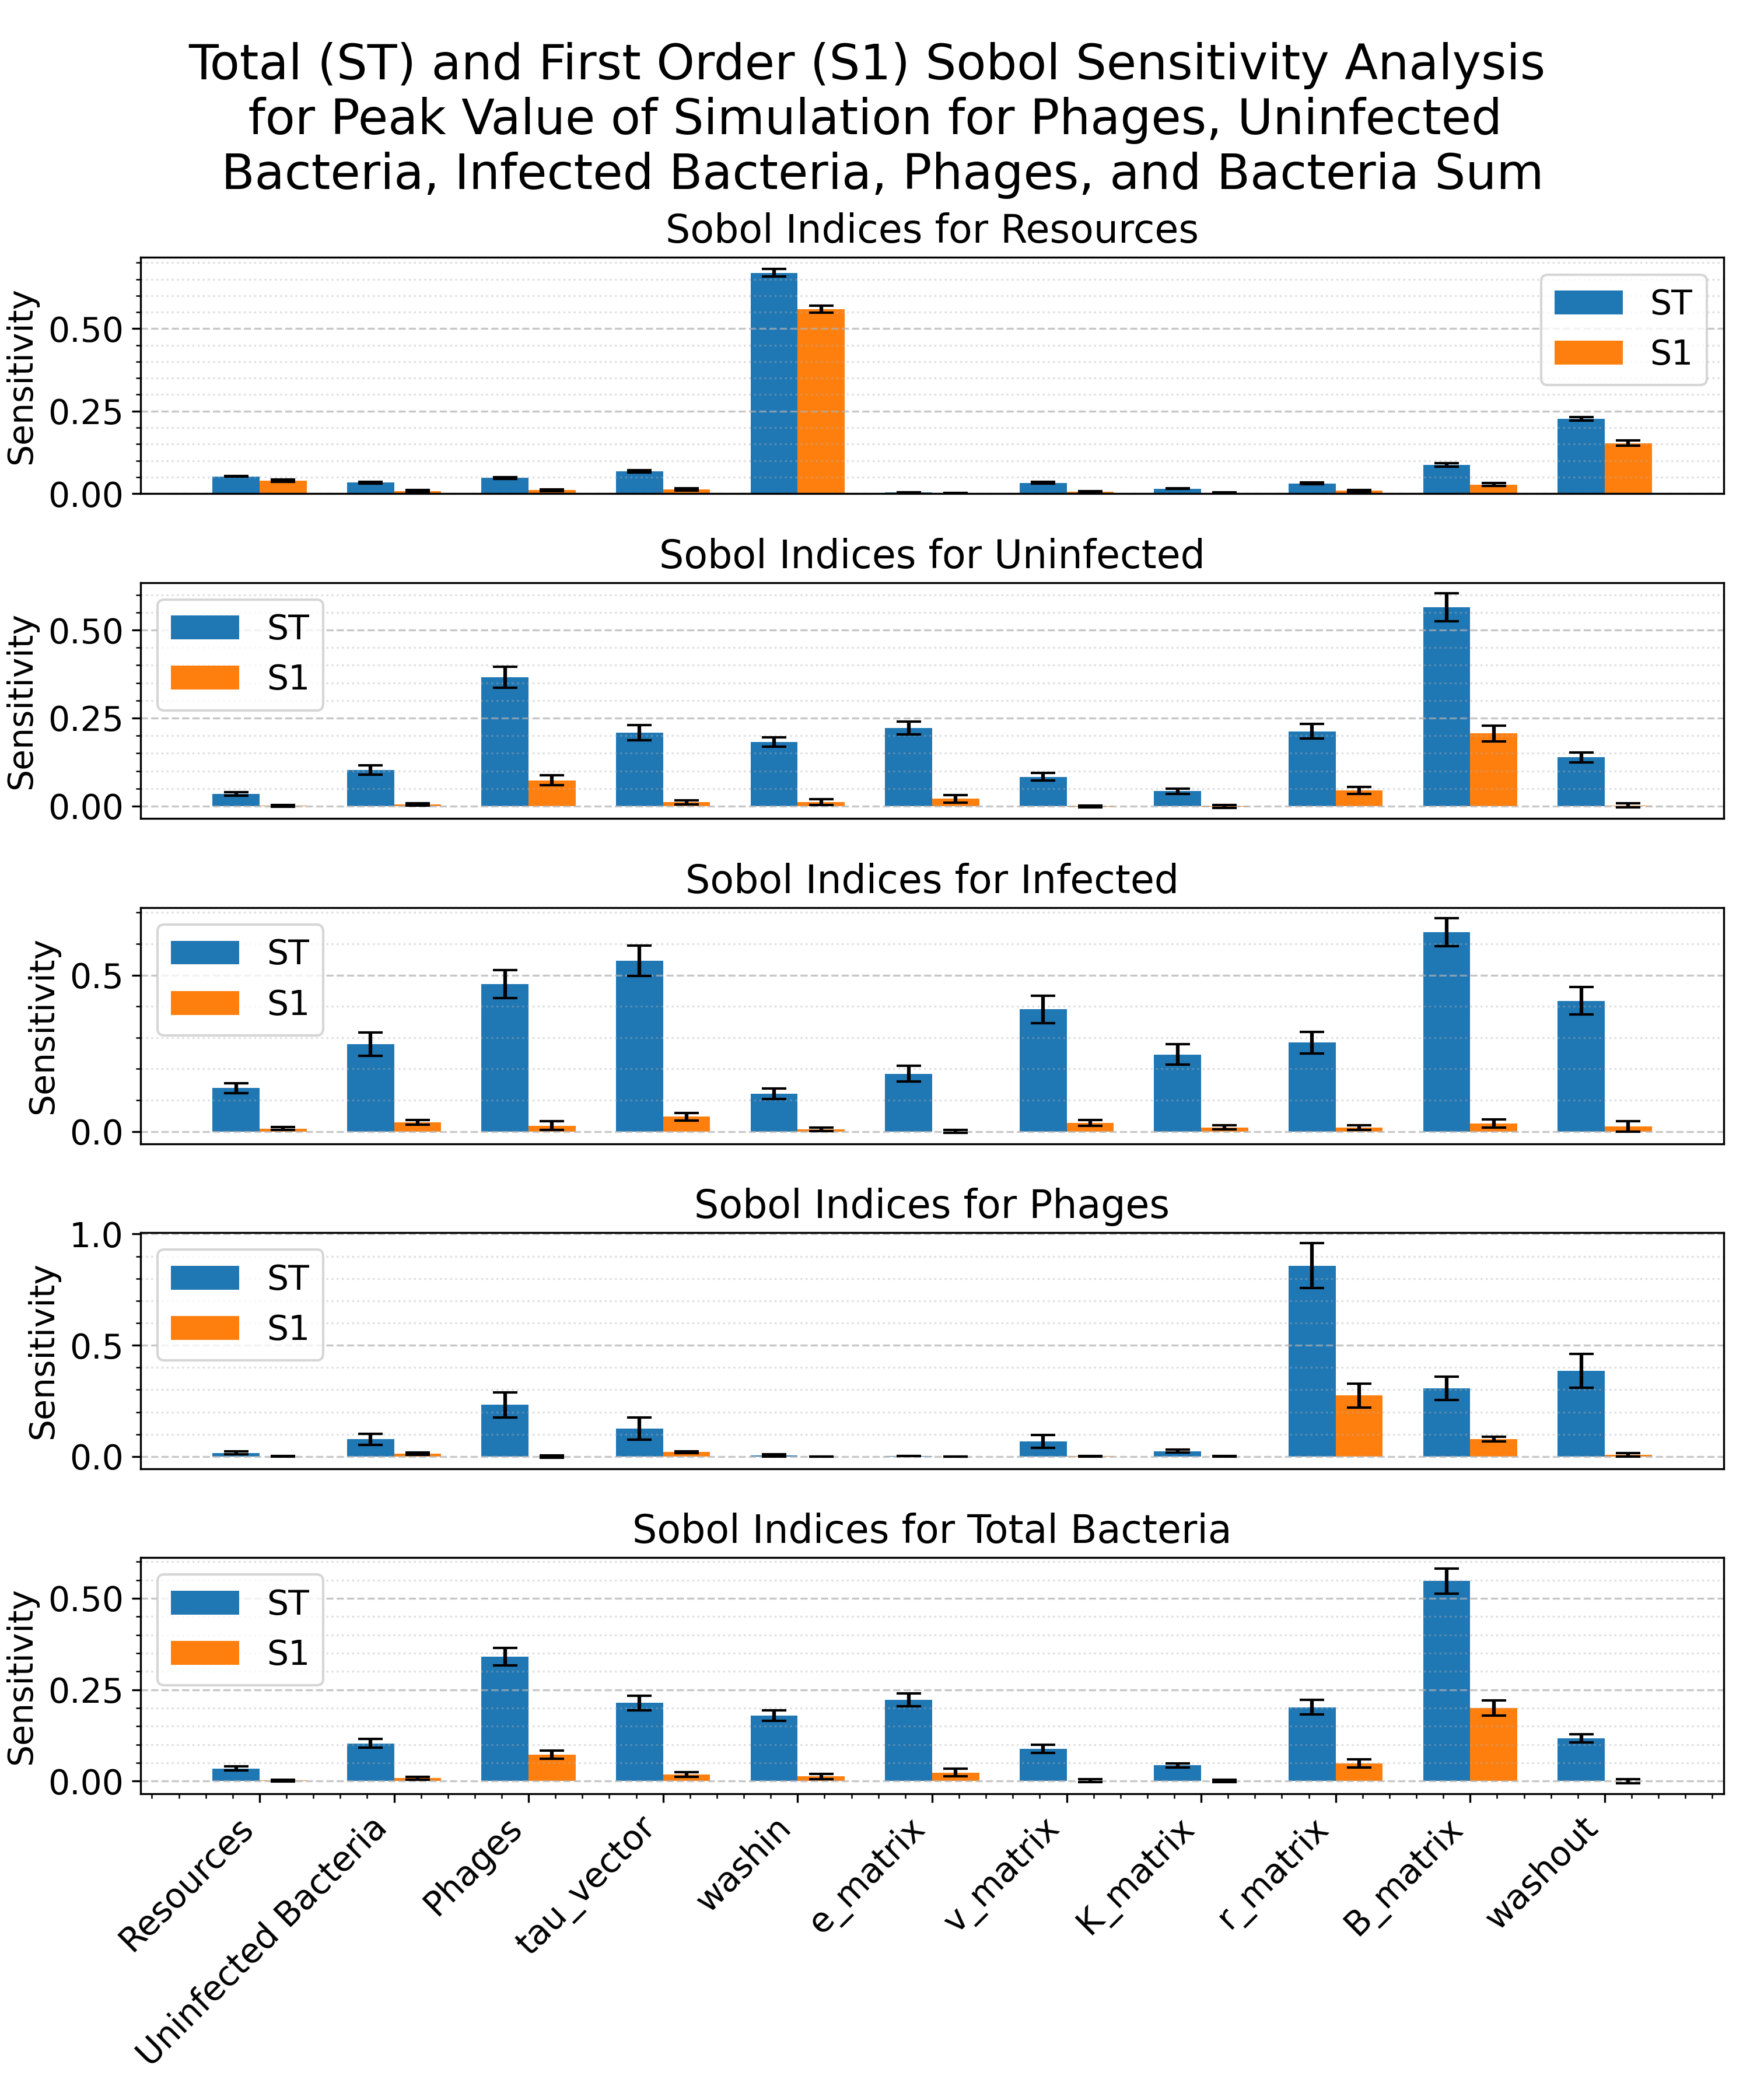
\includegraphics[width=\linewidth]{Plots/Created/SOBOL/SOBOL_analysis_1748084143_Peak.png}
        \caption{
            Peak population value. 
        }
        \label{fig:created:SOBOL_peak}
    \end{subfigure}
    \hfill
    \begin{subfigure}{0.32\linewidth}
        \centering
        \captionsetup{width=1\linewidth}
        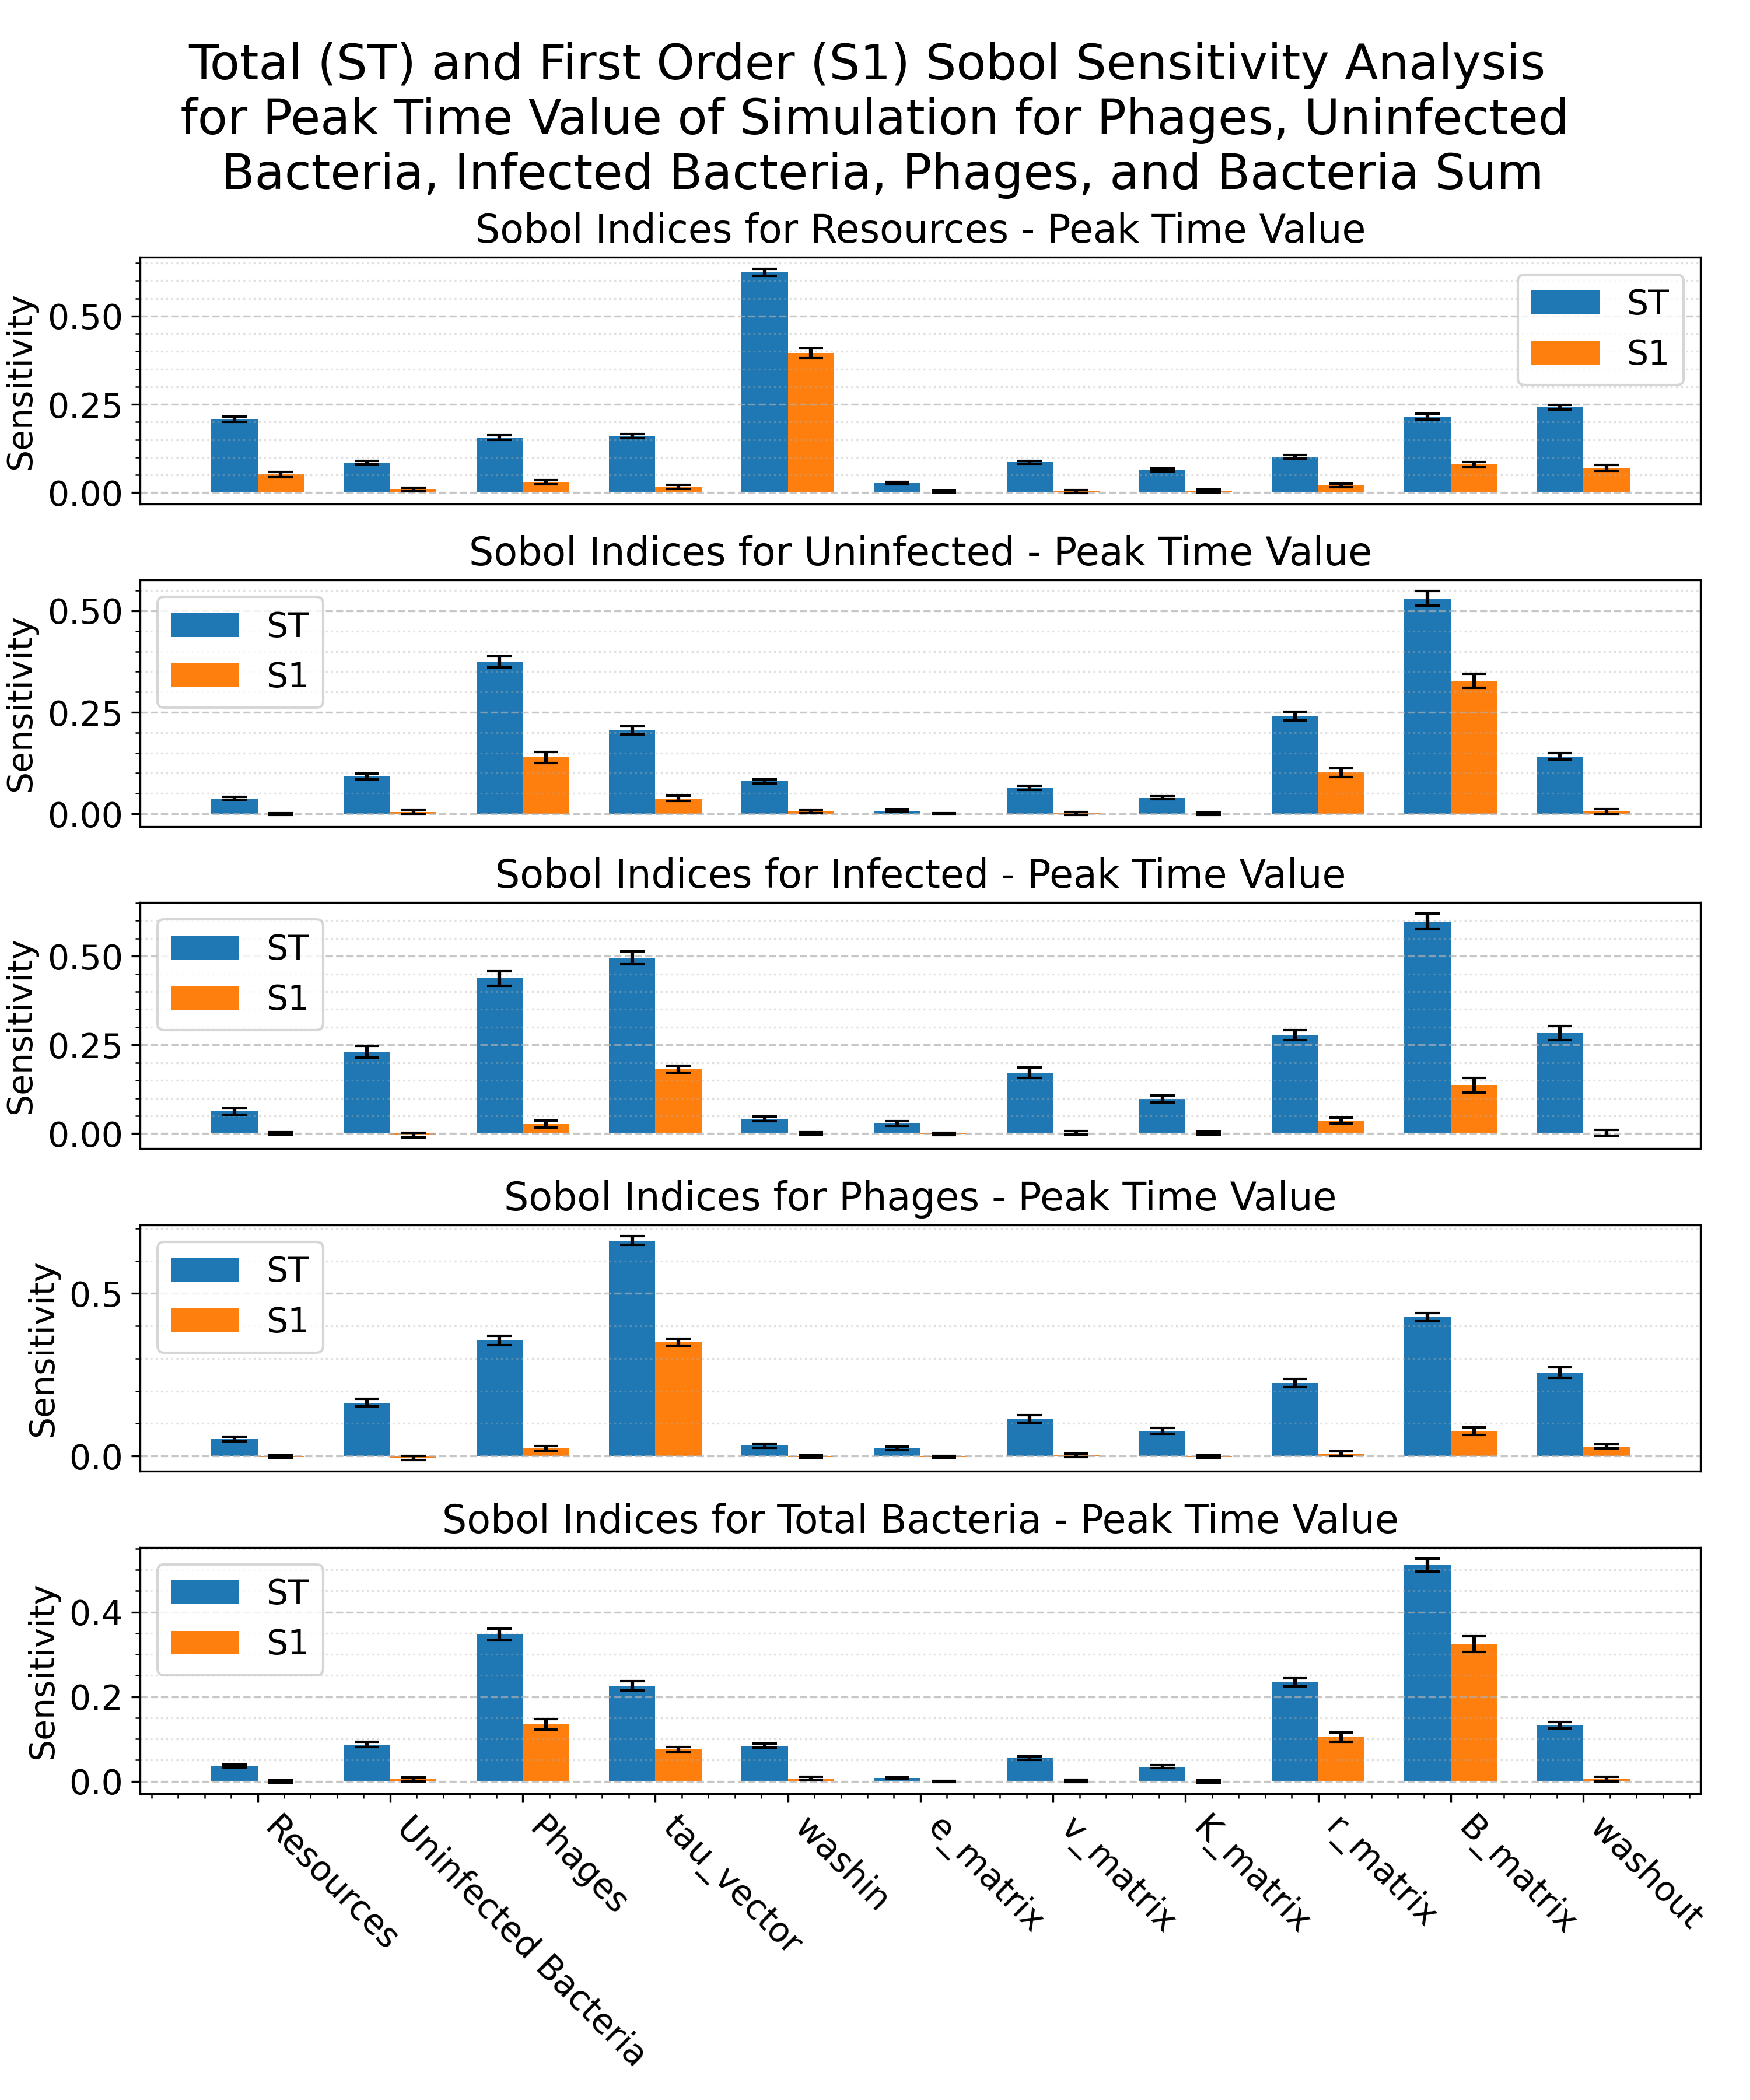
\includegraphics[width=\linewidth]{Plots/Created/SOBOL/SOBOL_analysis_1748084143_Peak_Time.png}
        \caption{
            Time at peak population. 
        }
        \label{fig:created:SOBOL_peak_time}
    \end{subfigure}
    \caption{
        SOBOL analyses for the average, peak, and peak time. 
        The data was saved from the dashboard and plotted using Matplotlib. 
        The average and variance analysis results were left out for nearly identical results to the final value. 
        The values used for this SOBOL test can be found in \Cref{tab:appendixE:SOBOL_analysis_values}. 
        The data used in \Cref{fig:created:SOBOL_final} was used for \Cref{fig:created:SOBOL_peak} and \Cref{fig:created:SOBOL_peak_time}. 
        The plot of the average and variance analysis can be found at \Cref{fig:created:SOBOL_average_extra} and \Cref{fig:created:SOBOL_variance_extra}
    }
    \label{fig:created:SOBOL_analyses}
\end{figure}

\subsection{Custom SOBOL Analysis - Peak Value and Peak Time}
Due to the similarity of the final, average, and variance value as seen in \Cref{fig:created:SOBOL_final}, \Cref{fig:created:SOBOL_average_extra}, and \Cref{fig:created:SOBOL_variance_extra} a custom SOBOL analysis that isn't included in the dashboard might result in a different SOBOL analysis result. 
To create the custom SOBOL analyses, the peak value and the time at the peak of the population is measured and analyzed. 
The peak is defined as the point where the population reaches 95\% of its absolute maximum value. 
The time at peak is measured at the point in time that the population reaches 95\% of the maximum value. 
This removes unintended side effects of the simulation. 
For populations that are only increasing in value, this prevents the measured peak from bunching up at the end of the simulation, skewing the data. 
As the peak is defined at 95\% of the absolute maximum value, populations that have a faster increase on population count at the end will have a time value closer towards the end of the simulation. 
For populations that reach a plateau, the 95\% rule will push the peak time towards the beginning of the simulation, while still "respecting" the absolute final value since $95\% \approx 100\%$. 
The 95\% rule can fail under certain situations, such as when there is cyclic behavior. 
See \nameref{sec:appendixF:why_95} for a more detailed explanation on why the 95\% rule is used. 

The results of the SOBOL peak and time at peak analyses can be seen in \Cref{fig:created:SOBOL_peak} and \Cref{fig:created:SOBOL_peak_time}. 
Although some of the bars between the final, peak, and time at peak values are the same, some are different. 
But overall, similar values can be seen across the the final, peak, and time at peak analyses. 
The peak infected values are more certain compared to the final infected values, which could be due to the 95\% rule removing some of the noise of the simulation. 
The time at peak values have less error compared to the final and peak value. 
This is due to the restricted range of values. The time at peak value can only fall somewhere between 0 and 15, the start and end values of the simulation respectively. 
The final and peak values can fall anywhere between 0 and any value, depending on the IC and how high the population can rise, and how fast the population can fall, \textit{if} the population count falls. 

\subsection{SOBOL Analysis - Without Washin and Washout}
In many of the plots, the washin and washout rate had a large influence on the final, peak, and time at peak value. 
\Cref{fig:created:SOBOL_no_wi_wo_extra} ran the same input as \Cref{fig:created:SOBOL_analyses}, but left the washin and washout rate out. 
The sensitivity plots for the final, average, variance, peak, and time at peak plots look different form one another. 
The final resource value depended heavily on the washin and washout rate, but without the washin and washout, the final resource depended heavily on the initial resource population. 
Since $S1 \approx ST$, the resource parameter does not depend on other higher order interactions. 

The peak value for the resources without washin and washout only depended on the initial resource consumption. 
Since there was no washin, no resources could be added, so the peak for the resources was always at $t=0$, and was dependent on the initial resource value. 
The time at peak value is always 0 as the resources are only being depleted, so no matter the change in parameter values, the parameter had no effect on the peak time, so SOBOL gives a value of 0 to every parameter for the resources. 
$\beta$ consistently had a large effect on the final, average, variance, peak, and time of peak value as 


\section{Initial Value Analysis Results}
\label{sec:results:initial_value_analysis}

The IVA section of the dashboard allows the user to visualize how a change in parameter value affects the population growth of the agents. 

In Figure 1 of \citet{mullaExtremeDiversityPhage2024}, they vary the initial concentration of bacteria and measure the time until bacterial collapse. 
The initial concentration value and time of collapse is plotted on the x and y-axis with a tight linear regression fit on the data. 
The observed logarithmic decrease suggests that the phage kinetics is adsorption-limited meaning that 
\Cref{fig:created:initial_value_analysis_UB_50_500_a_good_plot_2} replicates this graph. 

\Cref{fig:created:initial_value_analysis_UB_50_500_a_good_plot}, even considered a "good" curve, shows interesting behavior that diverges from that of \Cref{fig:created:initial_value_analysis_UB_50_500_a_good_plot_2}. 
Then though the behavior should be similar, changing other parameter values can alter how a parameter works. 
It would be expected that for10 initial uninfected bacteria and less the bacteria sum peak time would follow the linear regression line, but at around 100 uninfected bacteria and less, the peak curve goes horizontal. 
This suggests that something is restricting the bacterial growth. 

\begin{figure}
    \centering
    \begin{subfigure}{1\linewidth}
        \centering
        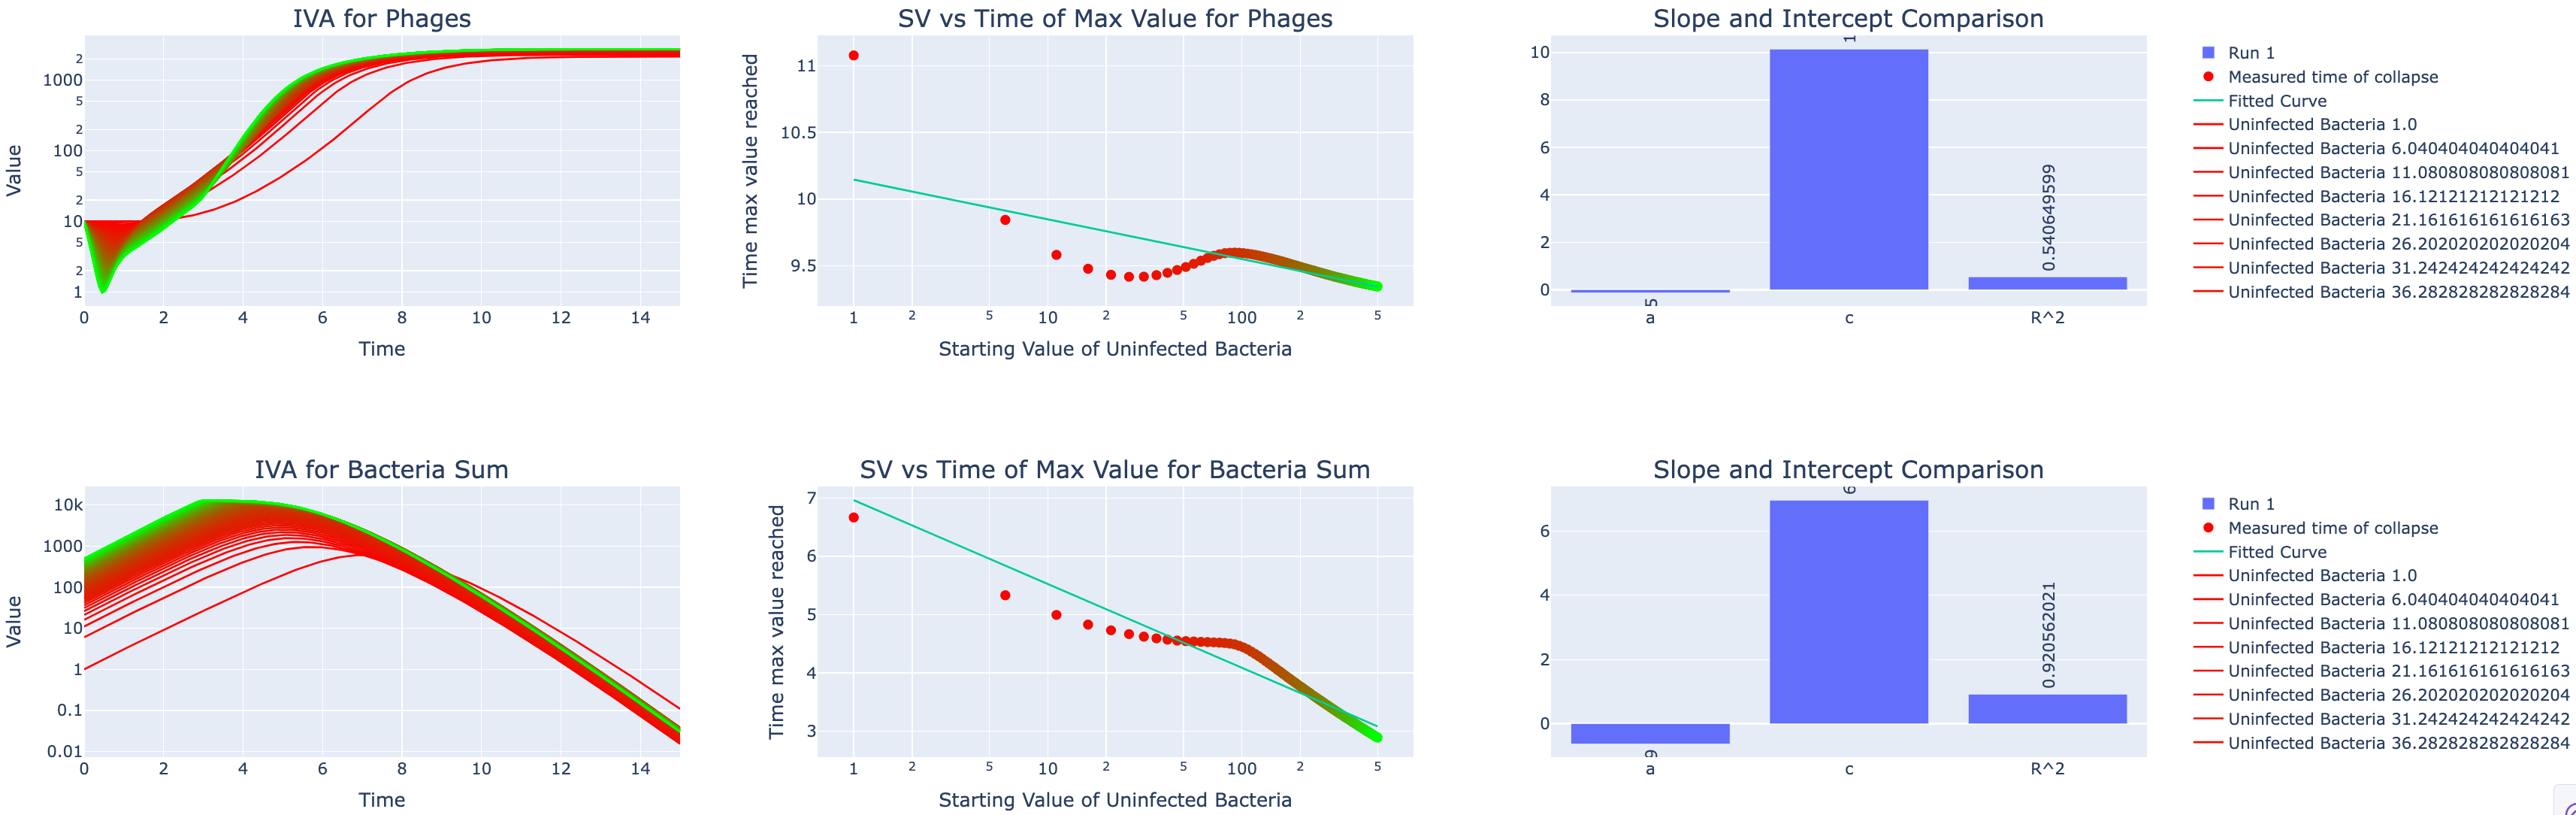
\includegraphics[width=\linewidth]{Plots/Created/IVA/initial_value_analysis_UB_50_500_a_good_plot.png}
        \caption{
            IVA for \Cref{tab:appendixE:a_good_curve}. 
            Replicates Figure 1 of \citet{mullaExtremeDiversityPhage2024}. 
        }
        \label{fig:created:initial_value_analysis_UB_50_500_a_good_plot}
    \end{subfigure}
    \hfill
    \begin{subfigure}{1\linewidth}
        \centering
        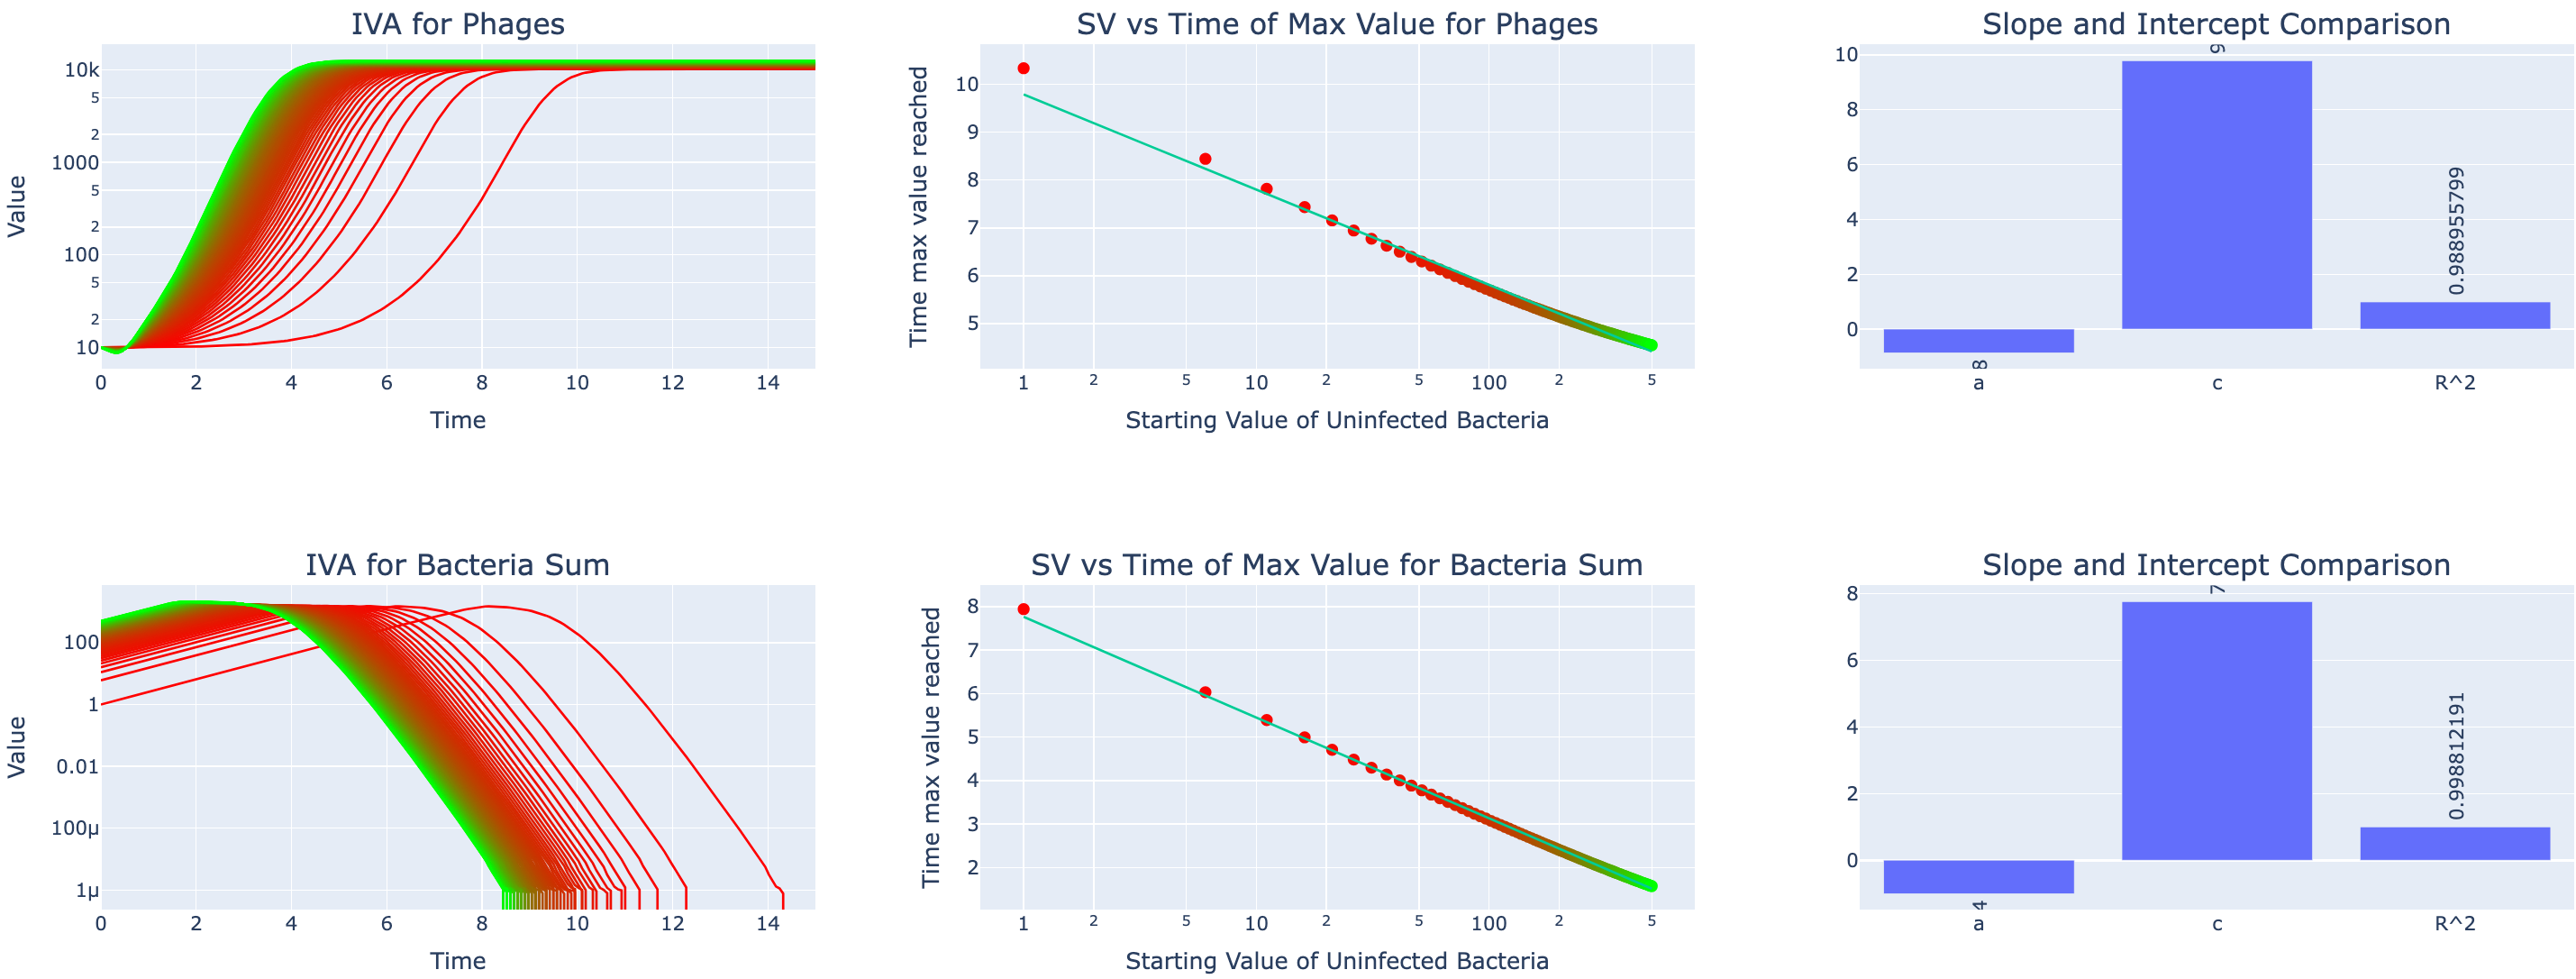
\includegraphics[width=\linewidth]{Plots/Created/IVA/initial_value_analysis_UB_50_500_a_good_plot_2.png}
        \caption{
            IVA for \Cref{tab:appendixE:a_good_curve_2}. 
            For uninfected bacteria less than 100, the phage-bacteria interaction is resource limited. 
            For 100 and higher, it is adsorption limited. 
        }
        \label{fig:created:initial_value_analysis_UB_50_500_a_good_plot_2}
    \end{subfigure}
    \caption{
        Varying initial Uninfected Bacteria concentration, from 50 to 500, with 30 unique values tested over two different instances of "good" curves. 
        Even with two "good" curves, even varying the default parameter values a tiny bit can have a large influence on how changing the initial bacteria concentration can have an influence on the dynamics of the system, changing the behavior of the peak time. 
        The default values for Figure a) and b) can be found at \Cref{tab:appendixE:a_good_curve} and \Cref{tab:appendixE:a_good_curve_2}. 
    }
\end{figure}